% In Rust programming, a reference is a pointer to reduce unnecessary movement of ownership. 
% One use case is where we pass reference to values to arguments of function. 
% If we pass owner to function, the owner is moved and the corresponding value is deallocated when the call of function ends. 
% To avoid this, the owner should always be returned. This may be an encumbrance while complex software system development. 
% By using reference, we do not have to worry about returning it, because reference is an additional pointer to an owned value. 
% Reference can be used for operation in the same way of owner, but also be moved without deallocation of value by keeping its owner live. 

% Reference is useful to avoid movement of ownership. However, one needs to track its lifetime and explicitly includes it in code, 
% because Rust compiler cannot infer it. This can be another encumbrance. We can instead acquire multiple owners to single value by using Reference Counting (Rc). 
% By leveraging Rc, a value can be shared like what borrowing plays the role in Rust programming. 
% The difference is that Rc checks number of owner pointing to the actual data and makes sure the data is not deleted 
% until all the owners are dereferenced. Using Rc is sometimes preferable approach for developers especially when lifetime planning is extremely difficult.
% However, the possible problem regarding to Rc is the cost for tracking the number of references. 
% Having this assumption, this experiment will show difference of behavior among Rc and simple reference.

In this experiment, CustomerBorrowed and CustomerRc are used to see difference of dropping time among reference and Rc. 
In the CustomerRc and OrderRc struct, all fields take Rc (Rc$<$T$>$). Similarly to the experiment in the last section, 
sets of integer, float, and String vector are created and their elements are borrowed or reference counted to create CustomerBorrowed or CustomerRc objects.
The dropping of objects deletes references or Rcs used for fields of the objects. However, it does not deallocate values to which they are pointing. 
Therefore, the evaluated runtime of dropping objects only consists of dropping time of reference or Rc, but deallocation time.
We generated 1, 1.5, 2, 2.5, 3, 3.5 million of CustomerBorrowed and CustomerRc objects and performed drop one by one. 

\subsection{Result}
Figure\ref{fig:rc_ref} shows comparison of runtime dropping CustomerBorrowed and CustomerRc objects. 
The result shows significant difference of dropping time among the two objects; deletion of CustomerRc is much slower than CustomerBorrowed. 
The runtime of dropping CustomerBorrowed is about 60 times faster than dropping CustomerRc. 

\begin{figure}[htb!]
    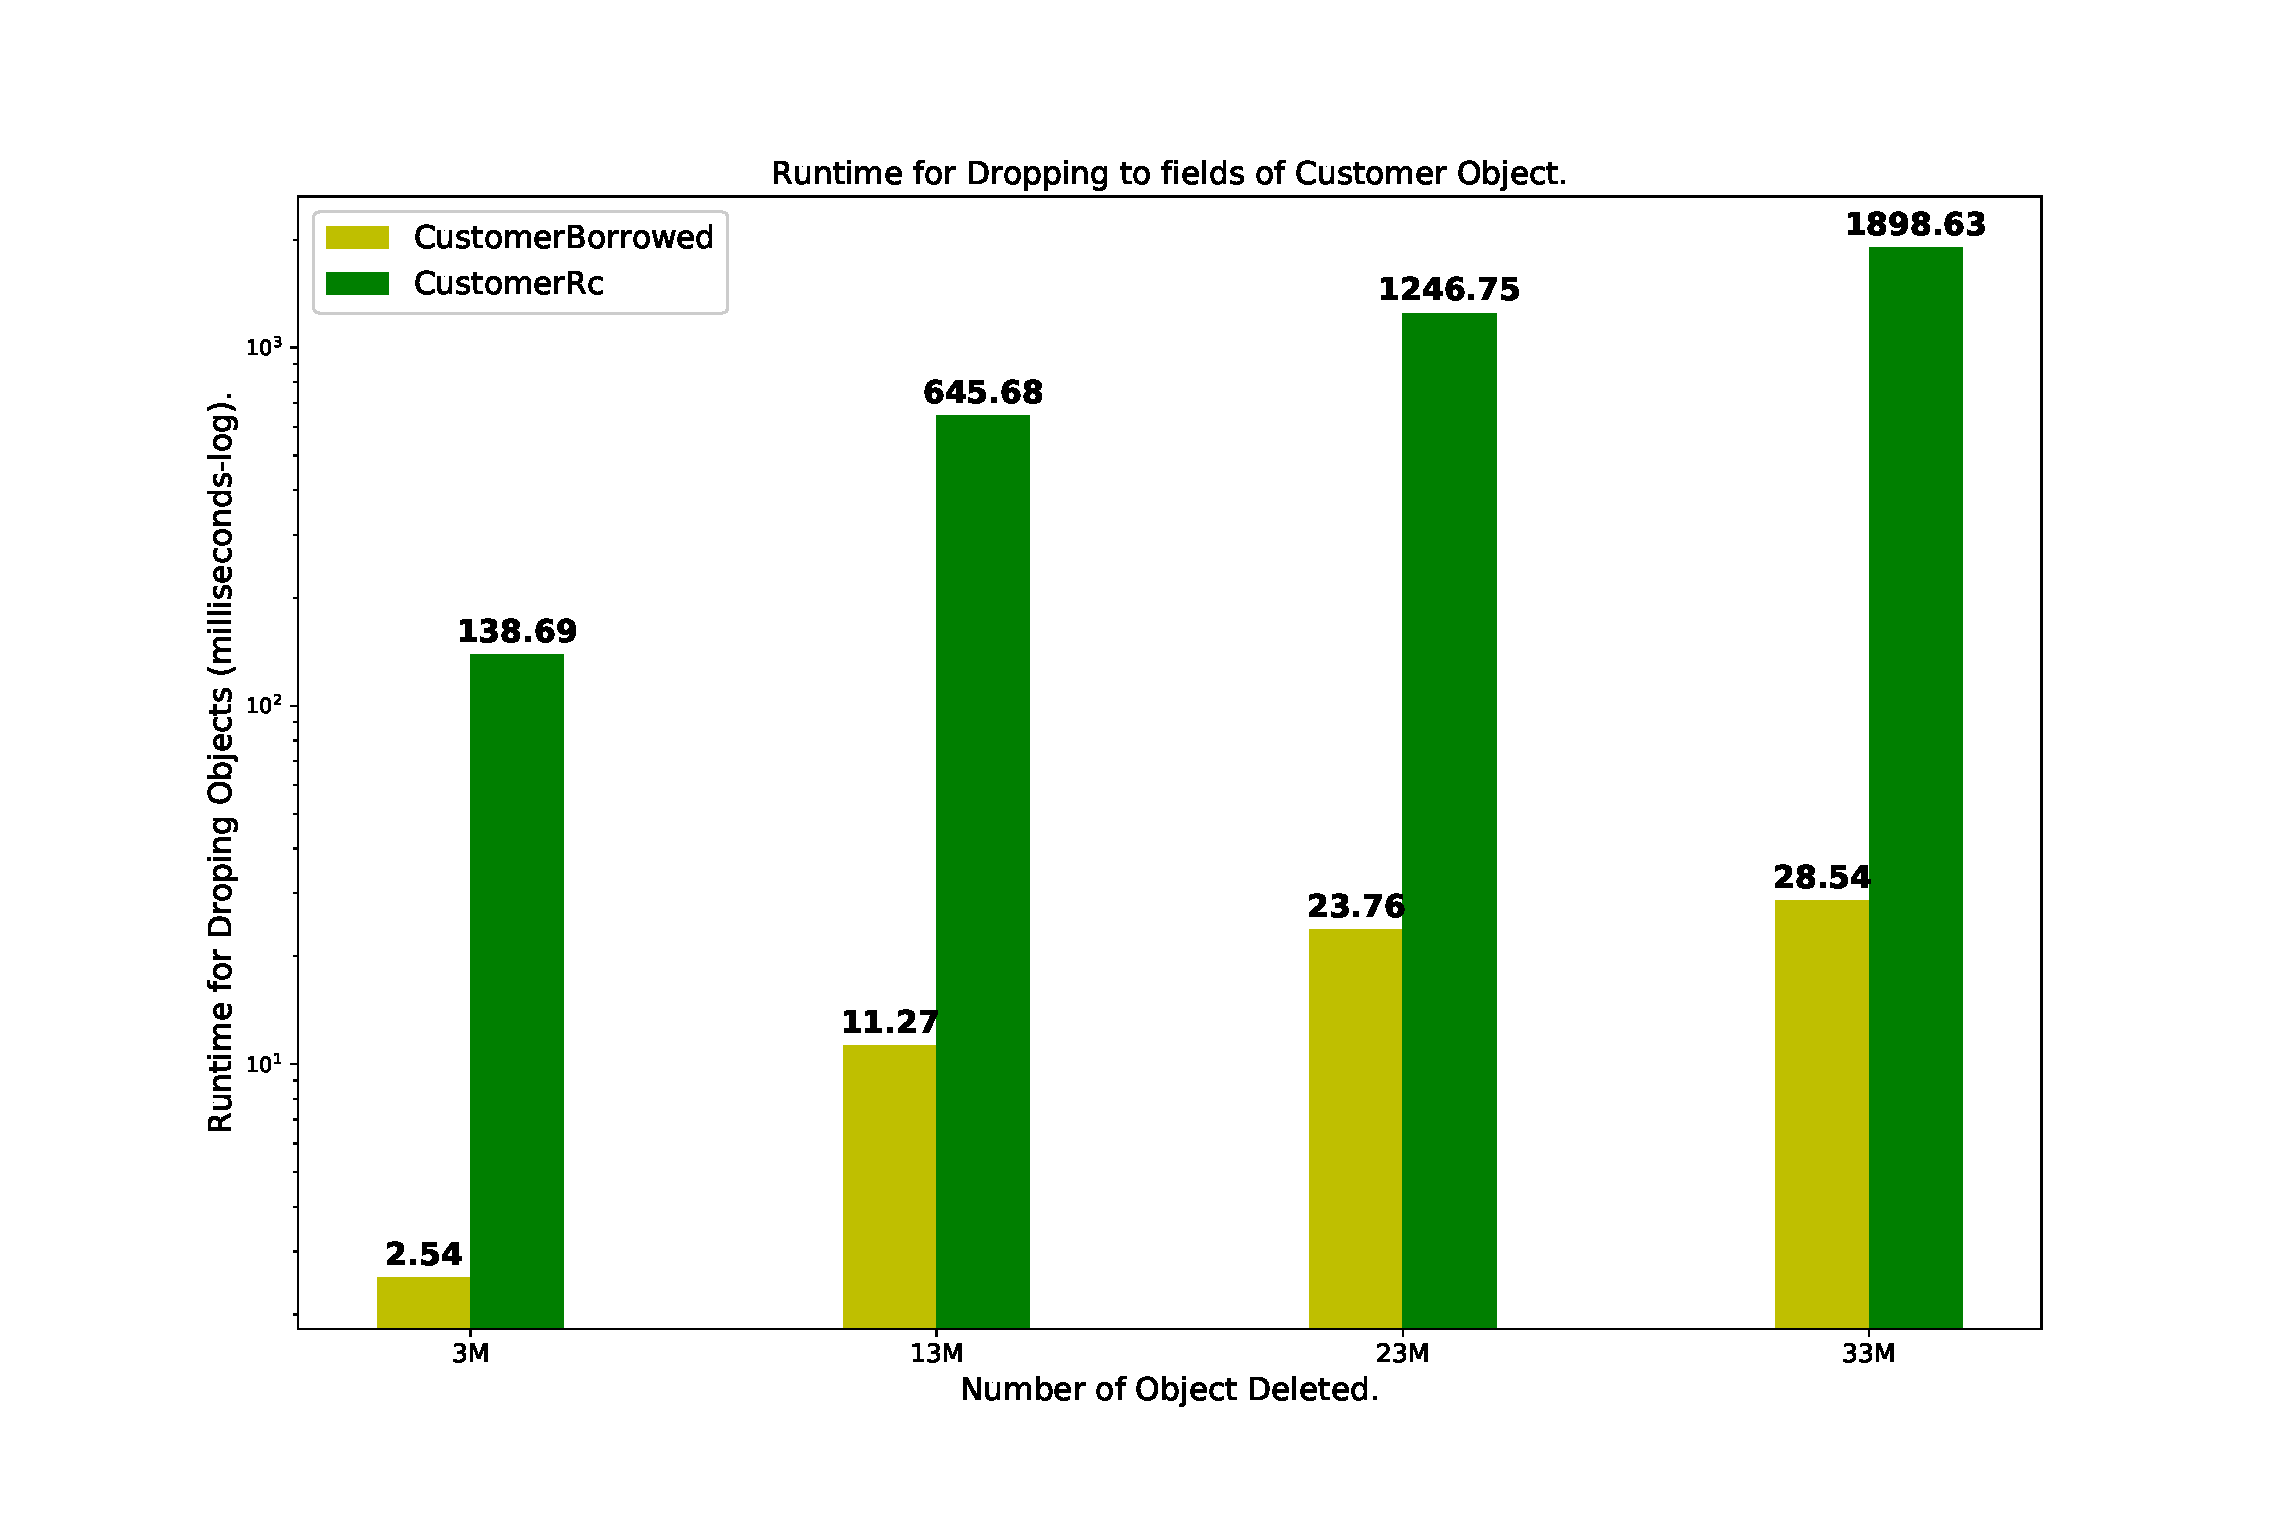
\includegraphics[width=15cm]{rust_droptime_borring_rc.eps}
    \caption{Runtime for dropping Customer Object}
    \label{fig:rc_ref}
\end{figure}


\subsection{Discussion}
In this experiment, an assessment is conducted to verify whether there is difference between behavior of reference and Rc.
The reason why dropping Rc is much slower than dropping reference is that Rc requires runtime overhead to check some states of the variable, 
but when to drop reference is already determined at compile time. When dropping Rc, Rc has to check the number of variable pointing to the actual content and decide 
deallocate the memory or not. However, memory management and lifetime strategy of reference is already determined at compile time.
This determination of memory management strategy at compile increases runtime performance of dropping complex object constructed with reference type variable.
This may say that we should use reference whenever high performance computation is critical.

However, dealing with reference is sometimes cumbersome. Tracking lifetime of reference can be done easily in simple situation. 
But, if we have complex objects constructed with fields of reference, the lifetime tracking become extremely difficult. 
For example, constructing nested objects with reference fields require a developer to plan memory management with many lifetime symbols. 
Using reference counting eliminates developer's responsibility to specify lifetime of variables. 
This may ease and speed up development process, and increase understandability of codes.

Even though we have stack allocated values, such as i32 and f64, in Rc in our experiment, 
one should avoid wrapping stack allocated values in Rc. Wrapping value in Rc allocates heap memory so that allocating Rc$<$i32$>$ or Rc$<$f64$>$ unnecessarily use space of 
heap. Additionally, stack allocated values are usually easy to be copied. Therefore, developer does not have to even use reference; one can just copy the value. 
Copying value in Rust is to copy the original value and to assign the copy to new owner variable. 